\documentclass[]{article}
\usepackage{lmodern}
\usepackage{amssymb,amsmath}
\usepackage{ifxetex,ifluatex}
\usepackage{fixltx2e} % provides \textsubscript
\ifnum 0\ifxetex 1\fi\ifluatex 1\fi=0 % if pdftex
  \usepackage[T1]{fontenc}
  \usepackage[utf8]{inputenc}
\else % if luatex or xelatex
  \ifxetex
    \usepackage{mathspec}
  \else
    \usepackage{fontspec}
  \fi
  \defaultfontfeatures{Ligatures=TeX,Scale=MatchLowercase}
\fi
% use upquote if available, for straight quotes in verbatim environments
\IfFileExists{upquote.sty}{\usepackage{upquote}}{}
% use microtype if available
\IfFileExists{microtype.sty}{%
\usepackage{microtype}
\UseMicrotypeSet[protrusion]{basicmath} % disable protrusion for tt fonts
}{}
\usepackage[margin=1in]{geometry}
\usepackage{hyperref}
\hypersetup{unicode=true,
            pdftitle={基因表达保守性强度的经验贝叶斯估计理论模型},
            pdfauthor={Jingwen Yang},
            pdfborder={0 0 0},
            breaklinks=true}
\urlstyle{same}  % don't use monospace font for urls
\usepackage{graphicx,grffile}
\makeatletter
\def\maxwidth{\ifdim\Gin@nat@width>\linewidth\linewidth\else\Gin@nat@width\fi}
\def\maxheight{\ifdim\Gin@nat@height>\textheight\textheight\else\Gin@nat@height\fi}
\makeatother
% Scale images if necessary, so that they will not overflow the page
% margins by default, and it is still possible to overwrite the defaults
% using explicit options in \includegraphics[width, height, ...]{}
\setkeys{Gin}{width=\maxwidth,height=\maxheight,keepaspectratio}
\IfFileExists{parskip.sty}{%
\usepackage{parskip}
}{% else
\setlength{\parindent}{0pt}
\setlength{\parskip}{6pt plus 2pt minus 1pt}
}
\setlength{\emergencystretch}{3em}  % prevent overfull lines
\providecommand{\tightlist}{%
  \setlength{\itemsep}{0pt}\setlength{\parskip}{0pt}}
\setcounter{secnumdepth}{0}
% Redefines (sub)paragraphs to behave more like sections
\ifx\paragraph\undefined\else
\let\oldparagraph\paragraph
\renewcommand{\paragraph}[1]{\oldparagraph{#1}\mbox{}}
\fi
\ifx\subparagraph\undefined\else
\let\oldsubparagraph\subparagraph
\renewcommand{\subparagraph}[1]{\oldsubparagraph{#1}\mbox{}}
\fi

%%% Use protect on footnotes to avoid problems with footnotes in titles
\let\rmarkdownfootnote\footnote%
\def\footnote{\protect\rmarkdownfootnote}

%%% Change title format to be more compact
\usepackage{titling}

% Create subtitle command for use in maketitle
\newcommand{\subtitle}[1]{
  \posttitle{
    \begin{center}\large#1\end{center}
    }
}

\setlength{\droptitle}{-2em}

  \title{基因表达保守性强度的经验贝叶斯估计理论模型}
    \pretitle{\vspace{\droptitle}\centering\huge}
  \posttitle{\par}
    \author{Jingwen Yang}
    \preauthor{\centering\large\emph}
  \postauthor{\par}
      \predate{\centering\large\emph}
  \postdate{\par}
    \date{2018-10-11}


\begin{document}
\maketitle

\section{转录组进化的稳定化选择压模型}

  在基因表达进化的过程中,OU模型认为,基因表达的变化会受到一个稳定的选择压力。这种模型相较于认为基因表达变化是一个随机过程的布朗运动模型而言更加符合基因表达变化的实际情况。

  OU模型有两个特点。

\begin{enumerate}
\def\labelenumi{\arabic{enumi}.}
\item
  给定基因的表达水平\(x\)存在一个最适合值\(\mu\)。当其表达值\(x\)等于或在最适值\(\mu\)附近时,该基因的适合度是最高的。而相对于基因表达而言,DNA序列水平的突变是一个随机的过程。突变的产生会使基因的表达发生改变,进而很大程度上偏离其表达最适值。
  也就是说,基因表达的变化受到序列突变(方差为\(\sigma^2\))的驱动,其适应度遵循一个高斯正态过程,其形式为
  \[f\left(x\right)=e^{-\frac{\omega\left(x-\mu\right)^2}{2}}\]
  其中\(\mu\)为基因\(x\)的表达最适值,\(\omega\)为作用于\(x\)的稳定选择压系数。当\(x=\mu\)时,其适应度\(f\left(x\right)\)达到最大值;\(x\)偏离\(\mu\)的程度越大,其适应度\(f(x)\)越小。稳定选择压系数\(\omega\)的大小反映了当\(x\)变化时,其适应度\(f(x)\)变化的快慢。当\(x\)受到的选择压系数\(\omega\)越大时,其适应度\(f(x)\)下降越快,反之,其适应度\(f(x)\)变化越慢。
\item
  基因表达水平\(x\)偏离最适值\(\mu\)后,回复到最适值\(\mu\)的过程受到正选择作用的影响;这种``回复作用力''的强度与该基因所收到的稳定化选择压强度\(\omega\)线性相关。
\end{enumerate}

  给定基因表达初始值\(x_0\),
经历\(t\)单位的进化时间后,OU模型预测\(x(t)\)的表达值遵循一个正态分布,其均值\(E[x|x_0]\)和方差\(V[x|x_0]\)分别表示为
\[E\left[x|x_0\right]=\mu\left(1-e^{-\beta t}\right)+x_0e^{-\beta t}\]

\[V\left[x|x_0\right]=1-\frac{e^{-2\beta t}}{W}\]
其中\(\beta=W\sigma^2\)表示表达的进化速度,\(W\)表示基因表达所受到的保守性强度,上述公式可简写为\(OU\left(x\left|x_0;\  \theta\right|\right)\),其中\(\theta=(\mu, \beta t, W)\)是参数向量。

  保守性强度(\(W\))对于反映基因表达所受到的稳定选择压强度\(\omega\)及其在进化过程中发生的变化(序列突变对表达水平产生的影响,方差为\(V_0\))起到十分重要的作用。本文的主要目的是构建估计基因表达在多物种进化过程中所受到的保守性强度(\(W\))的统计方法,此处我们主要用RNA-seq数据中的RPKM作为基因表达的主要度量方式。在物种的系统发生关系中,\(W\)的生物学含义表示为
\[W=\frac{4Ne \omega}{1-e^{-4Ne\omega V_0}}\]
其中\(Ne\)代表有效群体大小,\(V_0\)表示序列突变对表达水平产生的影响的方差。当选择压系数趋近于无穷时,\(W\approx4Ne\omega\);当选择压系数\(\omega\approx0\)时,\(W\approx1/V_0\)。

\hypertarget{ou}{%
\section{物种系统发生关系中的静态OU模型}\label{ou}}

  图一表示特定组织的比较转录组分析的进化关系,其包含两个过程。

\begin{enumerate}
\def\labelenumi{\arabic{enumi}.}
\tightlist
\item
  从组织起源结点\(Z\)到该组织物种分化结点\(O\)的进化谱系关系,该过程经历了\(\tau\)个进化时间单位。给定结点\(Z\)处的初始表达水平\(z_0\),基因的表达水平从结点\(Z\)处的\(z_0\)到结点\(O\)处的\(x_o\)的过程可用OU过程表示为\(OU(x_o|z_0;\theta)\),\(\theta\)表示参数向量\(\theta=(\mu, \beta \tau, W)\)。
\item
  从该组织的物种分化结点\(O\)到当前\(n\)个物种的进化谱系关系,该过程经历了\(t\)个进化时间单位。当前\(n\)个物种的基因表达水平表示为\(\boldsymbol{x}=(x_1,\cdots,x_n)\)。在给定结点\(O\)的表达水平\(x_o\)的条件下,当前\(n\)个物种表达水平的联合概率密度可用\(P(\boldsymbol{x}|x_o)\)表示,并可用OU过程推导。\(P(\boldsymbol{x}|z_0)\)表示在给定组织起源结点结点\(Z\)的表达水平\(z_0\)的条件下,当前\(n\)个物种表达水平的联合概率密度,其可表示为
  \[P(\boldsymbol{x}|z_0)=\int_{-\infty}^{\infty}OU\left(x_o|z_0;\tau\right)P\left(\boldsymbol{x}|x_o\right)dx_o\]
\end{enumerate}

\begin{figure}
\centering
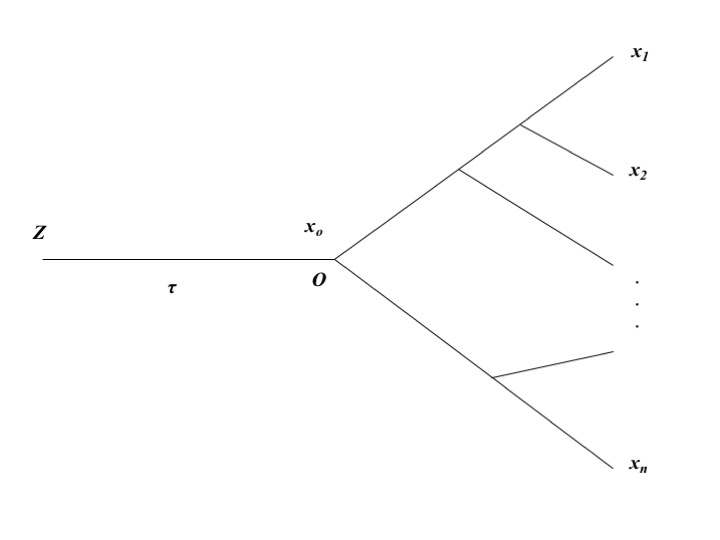
\includegraphics[width=0.7\textwidth,height=0.7\textwidth]{/blog/2018-10-11-W的经验贝叶斯估计_files/Figure1.jpg}
\caption{图一 比较转录组分析的进化关系图}
\end{figure}

  Hansen and
Martins指出\(P(\boldsymbol{x}|z_0)\)符合一个多元正太分布,其性质可由均值向量\(\boldsymbol{\mu}\)
和方差-协方差矩阵\(\boldsymbol{V}\)决定。但是当前物种的转录组信息包含太少的从结点\(Z\)到结点\(O\)的基因表达变化信息,这使得方差-协方差矩阵\(\boldsymbol{V}\)变得异常复杂。此外,一般的OU过程允许基因在不同物种中具有不同的基因表达变化速度\(\beta\)与表达保守性强度\(W\),在实际的分析过程中往往会出现过度参数化现象,导致统计自由度不足,给计算带来困难。

  为了解决这些技术上的问题,我们提出了静态OU(sOU)模型的概念。我们假定,特定组织的转录组整体的生物学功能在物种进化过程中是保守的。sOU模型主要包含两个方面的假设:

\begin{enumerate}
\def\labelenumi{\arabic{enumi}.}
\tightlist
\item
  图一中特定组织的起源结点\(Z\)发生在相当古老的时间之前,结点\(Z\)到该组织产生物种分化的结点\(O\)的进化时间\(\tau\)可近似认为\(\tau\approx+\infty\)。根据OU模型,我们可以得到结点\(O\)的表达均值等于其最适值\(\mu\),方差\(\rho^2=1/W\)。
\item
  基因表达水平在结点\(O\)处已达到稳定状态。结点\(O\)到当前物种的进化时间\(t\)相较于\(\tau\)是一个较短的进化过程。在这个过程中,基因表达的最适值\(\mu\)与保守性强度\(W\)保持不变。也就是说,基因表达的均值与方差在所有内部结点和外部结点中分别等于其表达最适值\(\mu\)和\(1/W\)。
\end{enumerate}

  在sOU模型下,\(P(\boldsymbol{x}|z_0)\)可作以下简化:

\begin{enumerate}
\def\labelenumi{\arabic{enumi}.}
\tightlist
\item
  因为进化时间\(\tau\)接近\(+\infty\),当前物种的表达水平\(\boldsymbol{x}\)几乎不受\(z_0\)的影响,因此可认定\(z_0\)与当前物种的表达水平\(\boldsymbol{x}\)相互独立,即\(P(\boldsymbol{x}|z_0) \approx P(\boldsymbol{x})\)
\item
  \(P(\boldsymbol{x}|z_0)\)的均值向量\(\boldsymbol{\mu}\)为一个统一的值。
\item
  基于前文的假设,不同物种基因表达变化的方差\(\rho^2=1/W\)。\(P(\boldsymbol{x}|z_0)\)的方差-协方差矩阵表示为\(\boldsymbol{V}=\boldsymbol{R}/W\),\(\boldsymbol{R}\)为当前物种基因表达的相关系数矩阵。
\end{enumerate}

  由于我们的主要目的是想计算不同基因的表达保守性强度\(W\),所以\(x\)的联合概率密度函数可表示为\(P(\boldsymbol{x};\mu,\boldsymbol{R}, W)\)

\hypertarget{w}{%
\section{\texorpdfstring{不同基因的\(W\)变化}{不同基因的W变化}}\label{w}}

  Gama分布的概率密度函数可表示为
\[f\left(x,\beta,\alpha\right)=\frac{\beta^{\alpha}}{\Gamma\left(\alpha\right)}x^{\alpha-1}e^{-\beta x}\]
其中,Gamma分布中的参数\(\alpha\)称为形状参数(shape
parameter),\(\beta\)称为尺度参数(scale
parameter)。Gamma分布的均值\(E[x]=\beta/\alpha\),方差\(V[x]=\beta/\alpha^2\)。

  sOU模型假定特定基因的保守性强度\(W\)在不同物种中为一固定的常数,而\(W\)在不同基因中均有不同。
在这里,我们引用Gamma分布的概,假定不同基因的保守性强度\(W\)作为一个随机变量服从Gamma分布,表示为:

\[\phi\left(W;\alpha,\overline{W}\right)=\frac{(\alpha/\overline{W})^\alpha}{\Gamma\left(\alpha\right)}W^{\alpha-1}e^{-\alpha W/\overline{W}}\]
其中\overline{W}为Gamma分布的均值,\(\alpha\)为形状参数(shape
parameter),\(\alpha/\overline{W}\)为尺度参数(scale parameter)。
当\(\alpha\)值很小时,\(W\)的变异度很高;当\(\alpha\rightarrow\infty\)时,\(W\)为一常数。

  \(\boldsymbol{x}=(x_1,\cdots,x_n)\)表示当前物种的基因表达水平,在OU模型下,\(\boldsymbol{x}\)的联合概率密度\(P(\boldsymbol{x;\mu,V})\)服从多元正太分布,可表示为
\[P\left(\boldsymbol{x,\mu,V}\right)=\frac{1}{\left(\sqrt{2\pi}\right)^n\left|\boldsymbol{V}\right|^{\frac{1}{2}}}\exp\left\{-\frac{\left(\boldsymbol{x}-\boldsymbol{\mu}\right)'\boldsymbol{V}^{\left\{-1\right\}}\left(\boldsymbol{x}-\boldsymbol{\mu}\right)}{2}\right\}\]
其中,\(\boldsymbol{\mu}\)为均值向量,\(\boldsymbol{V}\)为方差-协方差矩阵。在sOU模型下,方差-协方差矩阵\(\boldsymbol{V}=\boldsymbol{R}/W\)。将\(W\)作为一个随机变量,我们可以将\(\boldsymbol{x}\)的联合概率密度\(P(\boldsymbol{x};\boldsymbol{\mu},\boldsymbol{R},W)\)改写为\(P(\boldsymbol{x}|W;\boldsymbol{\mu,R})\)

\[
\begin{align*} 
P\left(\boldsymbol{x}|W;\boldsymbol{\mu,R}\right)&=\frac{W^{\frac{n}{2}}}{\left(\sqrt{\pi}\right)^n\left|R\right|^{\frac{1}{2}}}\exp\left\{-W\left(\boldsymbol{x}-\boldsymbol{\mu}\right)'\boldsymbol{R}^{-1}\left(\boldsymbol{x}-\boldsymbol{\mu}\right)\right\}\\
&=A\exp\left\{-Q\left(x\right)W\right\}W^{\frac{n}{2}}
\end{align*} 
\]
其中\(Q(\boldsymbol{x})=(\boldsymbol{x}-\boldsymbol{\mu})^T\boldsymbol{R}^{-1}(\boldsymbol{x}-\boldsymbol{\mu})\),表示\(\boldsymbol{x}\)的二次方程,\(A\)为归一化常数\(A=\pi^{-\frac{n}{2}}\left|R\right|^{-\frac{1}{2}}\)。

  由此可推出\(P\left(\boldsymbol{x};\boldsymbol{\mu},\boldsymbol{R},\alpha,\overline{W}\right)\)边缘密度函数
\[
\begin{align*} 
P\left(\boldsymbol{x};\boldsymbol{\mu},\boldsymbol{R},\alpha,\overline{W}\right)&=\int_0^{\infty}P\left(\boldsymbol{x}|W;\  \boldsymbol{\mu};\boldsymbol{R}\right)\phi\left(W;\  \alpha,\overline{W}\right)dW\\
&=A\left(\frac{\overline{W}}{\alpha}\right)^{n/2}\left(\frac{\Gamma\left(n/2+\alpha\right)}{\Gamma\left(\alpha\right)}\right)\left(\frac{\alpha}{\alpha+Q\left(\boldsymbol{x}\right)\overline{W}}\right)^{n/2+\alpha}
\end{align*} 
\]

\hypertarget{w}{%
\section{\texorpdfstring{特定基因保守性强度\(W\)的经验贝叶斯估计}{特定基因保守性强度W的经验贝叶斯估计}}\label{w}}

\hypertarget{w}{%
\subsubsection{\texorpdfstring{\(W\)的后验概率}{W的后验概率}}\label{w}}

  我们用贝叶斯过程来预测给定基因的表达保守性强度\(W\)。根据贝叶斯法则,在基因表达水平\(\boldsymbol{x}\)条件下,基因的表达保守性强度\(W\)的后验概率可表示为
\[
\begin{align*} 
P\left(W|\boldsymbol{x};\boldsymbol{\mu},\boldsymbol{R},\alpha,\overline{W}\right)&=\frac{\phi\left(W;\alpha,\overline{W}\right)P\left(\boldsymbol{x}|W;\boldsymbol{\mu},\boldsymbol{R}\right)}{P\left(\boldsymbol{x};\boldsymbol{\mu},\boldsymbol{R},\alpha,\overline{W}\right)}\\
&=\frac{\left[\frac{\alpha}{\overline{W}}+Q\left(\boldsymbol{x}\right)\right]^{\frac{n}{2}+\alpha}}{\Gamma\left(\frac{n}{2}+\alpha\right)}W^{\frac{n}{2}+\alpha-1}e^{-\left[\frac{\alpha}{\overline{W}}+Q\left(\boldsymbol{x}\right)\right]W}
\end{align*} 
\]
可得\(P\left(W|\boldsymbol{x};\boldsymbol{\mu},\boldsymbol{R},\alpha,\overline{W}\right)\)服从Gamma分布,均值与方差可分别表示为
\[E\left[W|x\right]\  =\left[\frac{\alpha+\frac{n}{2}}{\alpha+Q\left(x\right)\overline{W}}\right]\overline{W}\]
\[Var\left[W|x\right]=\left[\frac{\alpha+\frac{n}{2}}{\left(\alpha+Q\left(x\right)\overline{W}\right)^2}\right]\overline{W}^2\]

\hypertarget{ewboldsymbolx}{%
\subsubsection{\texorpdfstring{对后验均值\(E[W|\boldsymbol{x}]\)的解析}{对后验均值E{[}W\textbar{}\textbackslash{}boldsymbol\{x\}{]}的解析}}\label{ewboldsymbolx}}


\end{document}
